\documentclass{article}
\usepackage{amsmath}
\usepackage{amssymb}
\usepackage{graphicx}
\usepackage{tikz,pgfplots}
\usepackage{polynom}
\pgfplotsset{compat=1.18}
\usepackage{afterpage}


\begin{document}
   \begin{titlepage}
       \centering
       {
\includegraphics[width=0.2\textwidth]{logo.png} \par}
       {\bfseries\LARGE\textit{Universidad Nacional Autónoma de México}\par}
       \vspace{1cm}


       {\scshape\Large Facultad de Estudios Superiores Acatlán \par}
       \vspace{3cm}
      
       {\scshape\Huge Ejercicio 4: Bairstow \par}
       \vspace{3cm}


       {\slshape\Large Materia: Métodos Numéricos \par}
       \vfill


       {\Large Autor:Autor: Díaz Valdez Fidel Gilberto \par}
       {\Large Número de cuenta: 320324280 \par}
       \vfill


       {\slshape Octubre 2023\par}




   \end{titlepage}


\section{Propósito}
Durante el transcurso de este ejercicio en particular se tratará de ganar soltura,
entendimiento y rapidez en la utilización del método Bairstow. Será necesario tener
nociones básicas sobre cómo funcionan las operaciones matriciales, además del
conocer la fórmula general para la obtención de raíces tanto complejas como reales
para un binomio cuadrado dado.


\section{Instrucciones}
Según el polinomio siguiente: $$P(x) = x^5 -4.1x^4 + 3.35x^3 -4.775x^2 -2.6x +46.5$$
Obtener las raíces con las siguientes reglas o convenciones:
\begin{itemize}
   \item Tomar como valores iniciales $r = 1$, $s = 3$ para la primera aplicación.
   \item En la segunda aplicación tomar a $r = -1 $ y $s = -3$.
   \item Tolerancia al paro es del $0.5\%$ para el error relativo porcentual.
\end{itemize}


\section{Planteamiento}
Realmente en este ejercicio no hay muchas cosas ha tener en cuenta, esto debido a
que se nos está diciendo desde el principio los valores a escoger para la descomposición
del polinomio.


Lo que considero importante recalcar es el porque se nos otorgan datos
para dos aplicaciones. Esto es necesario porque sabemos que descompondremos el polinomio en
un binomio cuadrado a la vez, por lo tanto al tener un polinomio de grado $5$ en la
primera aplicación este se descompondrá en uno de grado $3$ y grado $2$ donde estaremos
en condiciones para encontrar la raíz del binomio cuadrático por medio de la fórmula
general, pero esto no sucede con el polinomio de grado $3$, por lo que será necesario
descomponerlo, es decir, volver a aplicar el método.


Una vez descompuesto el polinomio de grado $3$, se deberá haber descompuesto en dos,
un binomio cuadrático y en otro binomio, por lo que ya no será necesario volver a
hacer uso del método.


Por otra parte también considero de importancia ver cómo se comporta la gráfica,
ya que a través de está podemos darnos una idea de cuántas raíces reales y cuántas
complejas podemos esperar y aspirar a encontrar.


\section{Gráfica}
Tomaremos al polinomio inicial como una función en base a la variable $x$ para observar
su comportamiento.


\begin{figure}[h]
   \centering
   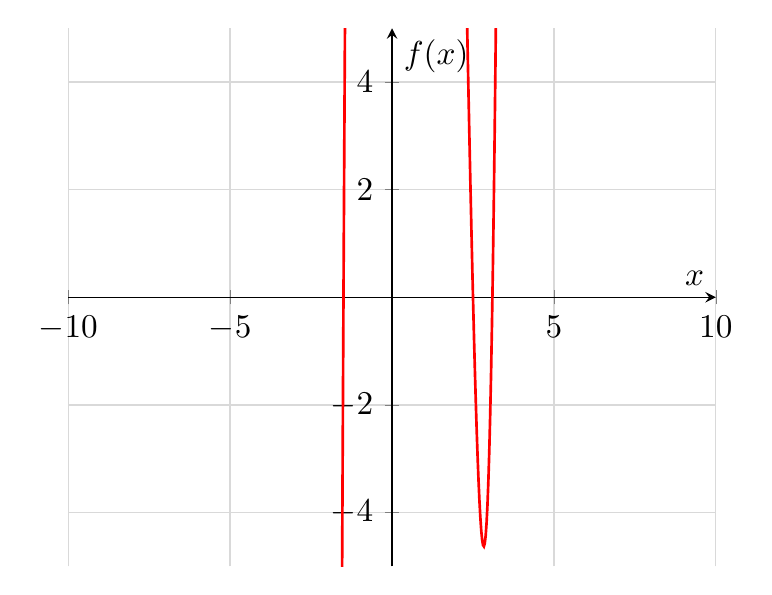
\begin{tikzpicture}[scale=1.2]
       \begin{axis}[
         axis lines= middle,
           xlabel=$x$,
           ylabel=$f(x)$,
           xmin=-10, xmax=10,   % Amplía los límites del eje x
           ymin=-5, ymax=5,     % Ajusta los límites del eje y según tus datos
           grid=major,  % Activa la cuadrícula
           grid style={gray!30},  % Estilo de la cuadrícula
           ]
           \addplot[domain=-2:3.5, samples=200, color=red, thick]{x^5 -4.1*x^4 + 3.35*x^3 -4.775*x^2 -2.6*x +46.5};
       \end{axis}
   \end{tikzpicture}
\end{figure}


Como se puede observar en la gráfica, solo se pueden detectar tres intersecciones
con el eje de las $x$ por lo que es probable que solo se nos presenten tres raíces
reales y las dos restantes sean complejas.


\section{Implementación del método}
Lo que debemos hacer para continuar es configurar nuestra hoja de cálculo de tal
manera que no se nos sea sencillo en todas las operaciones necesarias a realizar
para la obtención de las raíces.


Simplemente se deberá configurar para que se le otorguen tanto los coeficientes como
los datos iniciales de $r$ y $s$. También será necesario tener en cuenta las
operaciones matriciales para la obtención de los nuevos datos a evaluar.


Como se mencionó en el planteamiento, será necesario hacer uso del método más de
una vez debido a que se tiene un polinomio inicial de grado $5$ y también conocemos
que el método es capaz de descomponer el polinomio en uno cuadrático a la vez.


Por lo que en resumen tendremos que descomponer el polinomio inicial, utilizar la fórmula
general en el que encontramos, volver a descomponer el polinomio restante y hacer uso
de la fórmula general para encontrar las raíces del polinomio encontrado, por último
el polinomio restante después de la segunda implementación del método debe ser de
grado uno por lo que la raíz ya está encontrada.


Tal vez el hablar de esta manera presta a confusiones o pérdidas en el camino en
el transcurso de la idea, por esto trataré de mostrarlo de manera más gráfica.


\begin{equation}
   P(x) = x^5 + ax^4 +bx^3 +cx^2 +dx +f
\end{equation}


\begin{equation}
   P(x) = (x^2-rx-s)(x^3+ax^2+bx+c)
\end{equation}


\begin{equation}
   P(x) = (x^2-rx-s)(x^2-jx-k)(x + c)
\end{equation}


Como se puede observar en las ecuaciones descritas arriba, $1$ se tiene al polinomio
inicial, en $2$ se descompuso en dos polinomios, uno cuadrático y otro de tercer grado,
ese será el que deberemos volver a descomponer con la aplicación del método. Para la
tercera ecuación se puede observar a un polinomio descompuesto en dos cuadráticos y
uno de primer grado, como se explicó arriba, ahora solo restará hacer uso de la fórmula
general para las raíces de los binomios cuadráticos.


Donde $j$ y $k$ son variantes de $r$ y $s$ encontrados en la segunda aplicación del
método, la diferencia del nombre de las variables proviene del intento de evitar
confusiones con el método.


\section{Ejecución del Método}
\subsection{Primera Aplicación}
Una vez hemos planteado e implementado como debe comportarse el uso del método para este
polinomio en particular, ya nos encontramos en posición de pasar al uso del mismo teniendo
en cuenta lo que debería suceder y si no sucede como se planeaba, replantearse el modo
de ejecución.


Como bien ya hemos visto durante los ejercicios anteriores, el uso de las hojas de cálculo
son primordiales debido a que nos facilitan las operaciones y la implementación del método,
en nosotros queda con mayor peso la responsabilidad de haber planteado bien el problema
además claro de haberlo comprendido. Este caso no es la excepción, el planteamiento ya
lo hemos realizado y solo bastaría con configurar la hoja de cálculo para poder hacer
la aplicación del método.


Dentro de la hoja de cálculo se deberán encontrar operaciones matriciales, multiplicaciones,
sumas y es todo. Se deberá configurar a la hoja de cálculo para realizar divisiones sintéticas
específicamente dos por iteración de aplicación del método, además de las operaciones
matriciales para la obtención de los nuevos datos a probar.


Iteración 1. Primera obtención de polinomio cuadrático.


\begin{equation*}
   \begin{array}{c|ccccccc}
       & x^5 = 1 & x^4 = -4.1 &x^3 = 3.35 & x^2 = -4.775 & x = - 2.6 &x^0 = 46.5& \\
      &i = 5 & i = 4 & i = 3 & i = 2 & i = 1 & i = 0 & \\
       & 1 & -4.1 & 3.35 & -4.775& -2.6& 46.5 & \\
     r = 1 & & 1 &-3.1&3.25&-10.825&-3.675& \\
     s = 3 & & & 3 & -9.3 & 9.75 & -32.475 & \\
     \cline{2-8}
        & 1 & -3.1 & 3.25 & -10.825 & -3.675 & 10.35& b_i \\
   \end{array}
\end{equation*}


\begin{equation*}
   \begin{array}{c|ccccccc}
       &i = 5 & i = 4 & i = 3 & i = 2 & i = 1 & i = 0 & \\
       r = 1 & & 1 &-2.1&4.15&-12.975& & \\
       s = 3 & & & 3 & -6.3 & 12.45 &  & \\
       \cline{2-7}
         & 1 & -2.1 & 4.15 & -12.975 & -4.2 & c_i& \\
     \end{array}
\end{equation*}


Datos encontrados:


$b_1 = -3.674$, $b_0 = 10.35$, $c_1= -4.2$, $c_2 = -12.975$ y $c_3= 4.15$.


Con estos valores ya estamos en condiciones de encontrar los nuevos a usar:
\begin{equation*}
   \begin{bmatrix}
   c_2 & c_3\\
   c_1& c_2
   \end{bmatrix}
   \begin{bmatrix}
       \varDelta r \\
       \varDelta s
   \end{bmatrix}
   =
   \begin{bmatrix}
       -b_1\\
       -b_0
   \end{bmatrix}
   \rightarrow
   \begin{bmatrix}
       -12.975 & 4.15\\
       -4.2& -12.975
   \end{bmatrix}
   \begin{bmatrix}
       \varDelta r \\
       \varDelta s
   \end{bmatrix}
   =
   \begin{bmatrix}
       3.675  \\
       -10.35
   \end{bmatrix}
\end{equation*}


\begin{equation*}
   \begin{bmatrix}
       \varDelta r \\
       \varDelta s 
   \end{bmatrix}
   =
   \begin{bmatrix}
       -12.975 & 4.15\\
       -4.2& -12.975
   \end{bmatrix}^{-1}
   \begin{bmatrix}
       3.675  \\
       -10.35
   \end{bmatrix}
\end{equation*}


\begin{equation*}
   \begin{bmatrix}
       \varDelta r \\
       \varDelta s 
   \end{bmatrix}
   =
   \begin{bmatrix}
       -0.0254635003  \\
       0.8059303816
   \end{bmatrix}
\end{equation*}


Entonces se tiene que los nuevos valores de $r$ y $s$ son:
\begin{equation*}
   r = 1 - -0.0254635003 = 0.9745364997
\end{equation*}
\begin{equation*}
   s = 3 + 0.8059303816 = 3.805930382
\end{equation*}
Ahora tenemos que calcular el error porcentual relativo para asegurarnos de si se cumple
la tolerancia para otra iteración o no.


\begin{equation*}
  |\varepsilon_{rr}|= |\frac{\varDelta r}{r}| = 2.54635003\%
\end{equation*}
\begin{equation*}
   |\varepsilon_{rs}| = |\frac{\varDelta s}{s}| = 26.86434605\%
\end{equation*}


Cómo continúa sin cumplirse la tolerancia, debemos continuar la aplicación del método con
los nuevos valores de $r$ y $s$. En las próximas iteraciones ya no se pondrá el proceso
de manera tan gráfica, solo se continuará, insertando una tabla que contenga tantos los
datos obtenidos como su número de iteración.


\newpage
La tabla es la siguiente:


\begin{figure*}[h!]
   \centering
   \resizebox{9cm}{!} {
   \begin{tabular}{|c|c|c|c|c|}
       \hline
       Iteración   &   1   &   2   &   3   &   4   \\  \hline
       $b_5$   &   1   &   1   &   1   &   1   \\  \hline
       $b_4$   &   -3.1    &   -3.1255 &   -3.0999 &   -3.1    \\  \hline
       $b_3$   &   3.25    &   4.1101  &   4.0021  &   4   \\  \hline
       $b_2$   &   -10.825 &   -12.6649    &   -12.4043    &   -12.4   \\  \hline
       $b_1$   &   -3.675  &   0.7002  &   0.0115  &   0.0000  \\  \hline
       $b_0$   &   10.35   &   -1.0194 &   -0.0336 &   0.0000  \\  \hline
       $c_3$   &   4.15    &   5.8198  &   5.6544  &   5.65    \\  \hline
       $c_2$   &   -12.975 &   -15.1795    &   -14.6282    &   -14.625 \\  \hline
       $c_1$   &   -4.2    &   8.057   &   6.5991  &   6.5625  \\  \hline
       $r$     &   1   &   0.9745  &   1.0001  &   1   \\  \hline
       $s$     &   3   &   3.8059  &   3.7524  &   3.75    \\  \hline
       $\varDelta r$   &   -0.0255 &   0.0256  &   -0.0001 &   0.0000  \\  \hline
       $\varDelta s$   &   0.8059  &   -0.0536 &   -0.0024 &   0.0000  \\  \hline
       $\varepsilon_{rr}$  &   2.5464  &   2.6253  &   0.0121  &   0.0000  \\  \hline
       $\varepsilon_{rs}$  &   26.8643 &   1.4077  &   0.0627  &   0.0000  \\  \hline
   \end{tabular}
   }
\end{figure*}




Como se puede observar en la iteración número cuatro es donde se debe parar debido a que
se rompe con la tolerancia en ambos errores, con los datos de los coeficientes de $b$ y $c$
seremos capaces de descomponer el polinomio original de la siguiente manera:
\begin{equation*}
   P(x) = x^5 -4.1x^4 + 3.35x^3 -4.775x^2 -2.6x +46.5
\end{equation*}
\begin{equation*}
   P(x) = (x^2 - x -3.75)(x^3-3.1x^2-4x-12.4)
\end{equation*}


Por lo tanto ahora nuestro siguiente polinomio a descomponer es: $$(x^3-3.1x^2-4x-12.4)$$


\subsection{Segunda Aplicación}
El procedimiento será enteramente el mismo al descrito en la sección anterior, pero
ahora nos saltaremos la parte gráfica, ya que está ya debió quedar clara en la explicación
e implementación anterior hecha en la primera aplicación.


La diferencia radica en que como se nos dijo en las instrucciones, será obligatorio
comenzar con $r=-1$ y $s=-3$. Pasaremos directamente a la construcción de la tabla
y a la explicación de la misma.
\newpage
\begin{figure*}[h!]
   \centering
   \resizebox{12cm}{!} {
   \begin{tabular}{|c|c|c|c|c|c|c|c|}
       \hline
       $Iteracion$ &   1   &   2   &   3   &   4   &   5   &   6   &   7   \\  \hline
       $b_3$   &   1   &   1   &   1   &   1   &   1   &   1   &   1   \\  \hline
       $b_2$   &   -4.1    &   -2.9937 &   -3.1332 &   -3.1004 &   -3.1    &   -3.1    &   -3.1    \\  \hline
       $b_1$   &   5.1 &   1.224   &   0.0195  &   1.10E-03    &   0.00E+00    &   0.00E+00    &   0.00E+00    \\  \hline
       $b_0$   &   -5.2    &   -4.9122 &   0.3971  &   0.0021  &   0   &   0   &   0   \\  \hline
       $c_3$   &   1   &   1   &   1   &   1   &   1   &   1   &   1   \\  \hline
       $c_2$   &   -5.1    &   -2.8873 &   -3.1664 &   -3.1008 &   -3.1    &   -3.1    &   -3.1    \\  \hline
       $c_1$   &   7.2 &   -1.5408 &   -3.96   &   -3.9978 &   -4  &   -4  &   -4  \\  \hline
       $r$ &   -1  &   0.1063  &   -0.0332 &   -0.0004 &   0   &   0   &   0   \\  \hline
       $s$ &   -3  &   -2.4577 &   -4.0846 &   -4.0002 &   -4  &   -4  &   -4  \\  \hline
       $\varDelta r$   &   1.1063  &   -0.1395 &   0.0328  &   0.0004  &   0   &   0   &   0   \\  \hline
       $\varDelta s$   &   0.5423  &   -1.6268 &   0.0844  &   0.0002  &   0   &   0   &   0   \\  \hline
       $\varepsilon_{rr}$  &   1.1063  &   1.3123  &   0.9879  &   1   &   1   &   0.8244  &   0   \\  \hline
       $\varepsilon_{rs}$  &   0.1808  &   0.6619  &   0.0207  &   0   &   0   &   0   &   0   \\  \hline
   \end{tabular}
   }
\end{figure*}


Como se observa en la tabla, el momento en el que se deja de cumplir la tolerancia al error
relativo porcentual es en la 7ma iteración y los polinomios descompuestos son los siguientes:


\begin{equation*}
   P(x) = (x^3-3.1x^2-4x-12.4)
\end{equation*}
\begin{equation*}
   P(x) = (x^2 +0x +4)(x-3.1)
\end{equation*}


Con estos datos ya podemos descomponer el polinomio en su complitud teniendo como resultado esto:
\begin{equation*}
   P(x) = (x^2 - x -3.75)(x^2 +0x +4)(x-3.1)
\end{equation*}


Solo basta usar la fórmula general para encontrar las raíces tanto complejas como reales:


Primer binomio cuadrático:
\begin{equation*}
   (x^2 - x -3.75) \rightarrow x_1 = \frac{5}{2}, x_2 = -\frac{3}{2}
\end{equation*}


Segundo binomio cuadrático:
\begin{equation*}
   (x^2 +0x +4) \rightarrow x_1 = 2i, x_2 = -2i
\end{equation*}


Último polinomio:
\begin{equation*}
   (x-3.1) \rightarrow x = 3.1
\end{equation*}


Como habíamos analizado terminamos con 2 raíces imaginarias y 3 raíces reales, por lo que
podemos afirmar que logramos nuestro cometido y encontramos todas las raíces del polinomio
en cuestión.


\newpage


\section{Conclusión}
Definitivamente no se trata del método más sencillo de implementar, pero cumple su cometido
cuando se conoce y se analiza de manera detenida el entorno del problema para así lograr
utilizarlo y llevando cierto control debido a los resultados esperados acotados a través
del análisis previo.


Entre sus desventajas diría que se encuentra la facilidad que tiene para poder perderte
durante el proceso, pero esta se ve compensada con una tremenda ventaja, que es la facilidad
que se nos proporciona para encontrar todas las raíces de un polinomio, incluyendo las complejas
de una manera más sencilla que el método de Newton.


\end{document}


